\chapter{Курганы близ Лысой горы}

Сначала я узнал про курган во дворе дома на Перова, 25. Про него мне рассказала Настя, жившая там раньше неподалеку.

Это самая северная часть возвышенности Лысой горы. От упомянутой школы номер 180, переходим на север, в сторону Троещины, через улицу Серова. Склон начинает плавно понижаться в ту же сторону. Проходим мимо дома 23, и упираемся в курган слева от дома 25\footnote{Примерно в трехста метрах восточнее берега Радунки.}.

Жители окрестных девятиэтажек говорили, что это насыпанная кучей земля со снесенного Воскресенского кладбища. Я не знаю случаев, когда при сносе кладбища куда-то перемещают землю. Слободское кладбище, однако, находилось на месте домов по Перова 23, 23А, 30-Б, 30А – то есть внутри угла между Перова и Серова. Дом номер 25 – у северного края этого кладбища, а еще севернее по существовавшей прежде улочке стояли частные дома. Курган был между ними и кладбищем. Когда вокруг уже стояли многоэтажные дома, сильные дожди вымывали из кургана кости. Сейчас нельзя сказать, какую форму и размер он имел в давнее время.

\begin{center}
\includegraphics[width=\linewidth]{chast-gorodki/kurgany/s_IMG_20140806_125032.jpg}

\textit{Вид с бульвара Перова во двор.}
\end{center}

\begin{center}
\includegraphics[width=\linewidth]{chast-gorodki/kurgany/s_CRW_3890.jpg}

\textit{Вид на курган с севера.}
\end{center}


\begin{center}
\includegraphics[width=\linewidth]{chast-gorodki/kurgany/s_CRW_3892.jpg}

\textit{Вид на курган с востока.}
\end{center}


\begin{center}
\includegraphics[width=\linewidth]{chast-gorodki/kurgany/s_CRW_3894.jpg}

\textit{Вид на курган с юга.}
\end{center}


\begin{center}
\includegraphics[width=\linewidth]{chast-gorodki/kurgany/s_IMG_20140806_125336.jpg}

\textit{Вид с кургана на север.}
\end{center}

Метра три высотой, в буграх, но сохраняющий четкие рукотворные очертания. В 2016 году был изуродован велосипедистами, устроивших там себе трамплин.

Это может быть как самостоятельный древний погребальный курган (даже один из многих, постепенно замещенных более новыми, христианского времени могилами Воскресенской слободы), так и остатки древнего городища! Раньше левобережная часть Киева относилась к Черниговской губернии, Остёрскому уезду, а он славился и курганами, и городищами.

Рассматривая карту «Археологические памятники на территории Киева с древнейших времен до середины 1-го тысячелетия нашей эры» из книги «Киев: карты, иллюстрации, документы» 1982 года я увидел две отметки в снесенной ныне части села Выгуровщины, несколько на север от перекрестка бульвара Перова и проспекта генерала Ватутина. Обозначено: «отдельные находки трипольской культуры» и «отдельные находки скифского времени». Никаких более подробностей, но где скифы, там ведь и курганы.

Я исправно на протяжении нескольких лет наведывался к этому кургану, однако новые курганы там не вырастали, только машин вокруг больше парковалось. Словом, ничего больше узнать я не смог.

Но с некоторых пор я стал ездить на Лесной массив с Радужного через Воскресенку, по бульвару Перова. С улицы Петра Вершигоры ходит замечательная маршрутка, вроде сельских. В ней синие шторы, какие-то низкие лавки вместо сидений, и пахнет луком. Кажется, таких всего несколько на маршрут, оттуда до станции метро Лесная.

И вот я ездил и глядел в окно. 

Вдоль проспекта генерала Ватутина огибаем север Радужного массива, по дуге улицы Кибальчича (на север от которой, до нынешнего проспекта, еще в первой половине 20 века полумесяцем выгибалось болото Корчовня) выруливаем на прямой бульвар Перова – жилые дома стоят там близко к трассе, и вечером, через окна зданий, хорошо видны сценки из чужих жизней.

С Перова, не доезжая до Деснянской  водопроводной станции, маршрутка сворачивает налево, на восток, по проспекту Алишера Навои, который прорезает сосновый лес в пойме длинного водоема, русло коего стало болотом Куликовым и длинным прудом в парке Победы. Пойма осушалась и управлялась мелиоративными каналами, а один поныне исходит из упомянутого пруда, дабы исчезнуть в коллекторе близ роддома номер 6, ближе перекрестку Курнатовского и Петра Запорожца.

Но вернусь к повороту возле Перова. Сразу по левую руку, четной стороне Алишера Навои, пошли панельные кургузые девятиэтажки 92, 88, 84, 80. А позади них, перпендикулярно к улице, прячется ряд длинных пятиэтажек того же времени. Не хрущовки, а более долгие дома, обложенные белой плиткой.

Я вяло обращал внимание на то, что ближайший к улице ряд, там где девятиэтажки, стоит на невысоком, метров два с половиной, пригорке. Для удобства восхождения туда взбирается лестничка из бетонных плит.

Но что там, во глубине дворов – я не всматривался. Мимо проносилась свежая зелень деревьев, серо-бежевые стены домов с квадратами перекрытий. На плане РККА 1930-х, там есть возвышенность, причем частично вписывающаяся в ровный склон этого пригорка вдоль проспекта. 

Продолжая ездить, я приметил ложбину между девятиэтажкой номер 80 и длинным домом 76. Позади него к востоку – детская больница, тоже отвоевавшая кусок леса.

И однажды, вдруг я заметил то, что должно было броситься в глаза прежде всего. В проеме за девятиэтажками 84 и 80, между длинными домами 82 и 78, мелькнул зеленый курган.

Я мог крикнуть водителю маршрутки – стойте! Дело исторической важности! Окрыленно спрыгнуть со ступенек микроавтобуса, перебежать улицу, забуриться во дворы и бегать вокруг кургана, фотографируя его и делая замеры.

Но я продолжал, черт возьми, ездить мимо, всё собираясь как-нибудь туда отправиться и всё осмотреть.

Только в марте 2016-го я, за компанию с Алиной, отправился на местность.

Неряшливая карта поможет дальнейшему рассказу.

\begin{center}
\includegraphics[width=\textwidth]{chast-gorodki/kurgany/vosk-gorodishe.pdf}
\end{center}

Синее это бетонный канал. Около стоматологии он выходит из трубы и шурует через лес к подземному коллектору близ улицы Петра Запорожца. Вода из пруда в парке Победы (южнее через проспект, на карту не влез) течет по каналу на север.

Кружок с цифрой 3. Вообще всё зеленое на карте это сосновый лес. Местами он не обрывается так резко, как я нарисовал, но плавно сменяется пустырями. Тройкой отмечено кладбище домашних животных и окрестности. Около кладбища лес испахан какими-то неглубокими рвами (либо наоборот, невысокими валами), иногда сходящимися под прямым углом.

Это не лесная вспашка, когда лес высевают в обработанную таким образом землю, а либо остатки мелиоративных каналов, либо нечто другое. Окопы времен Великой Отечественной? Следы чего-то более давнего?

К сожалению, снимок за август 2016 года плохо передает рельеф:

\begin{center}
\includegraphics[width=0.80\textwidth]{chast-gorodki/kurgany/\myimgprefix IMG_20160815_124531.jpg}
\end{center}

Но вернемся к плану. Дома начиная от 92 по 80 стоят на пригорке, проспект – у подножия.

Бежевый фон не означает, что дворы голые и пустые, напротив, там много деревьев, да и не весь этот фон обозначает дворы. Лес плавно переходит в этот другой, смешанный вид местности.

Единицей в круге помечен предполагаемый курган. Прежде всего надо было убедиться, что это не бомбоубежище или какие-нибудь погреба, где люди хранят разную консервацию и мешки с картошкой.

Оказалось ни тем, и не другим, однако вероятно и не курганом. Поглядим сначала издалека, с нескольких ракурсов:

\begin{center}
\includegraphics[width=0.81\textwidth]{chast-gorodki/kurgany/\myimgprefix IMG_20160325_125723.jpg}

\textit{Слева – дом 80, справа – 78.}
\end{center}

\begin{center}
\includegraphics[width=0.81\textwidth]{chast-gorodki/kurgany/\myimgprefix IMG_20160325_130604.jpg}

\textit{Дом 80 стоит справа.}
\end{center}

\newpage

\begin{center}
\includegraphics[width=\textwidth]{chast-gorodki/kurgany/\myimgprefix IMG_20160325_125805.jpg}

\textit{Дом 82 – позади бугра.}
\end{center}

\begin{center}
\includegraphics[width=\textwidth]{chast-gorodki/kurgany/\myimgprefix IMG_20160325_125824.jpg}

\textit{Вид на северо-запад. Дом 82 – слева.}
\end{center}

\newpage

\begin{center}
\includegraphics[width=0.96\textwidth]{chast-gorodki/kurgany/\myimgprefix IMG_20160325_125927.jpg}

\textit{Юго-восточный угол бугра оказался прямоугольным. Слева – дом 78, справа – 80.}
\end{center}

\begin{center}
\includegraphics[width=0.96\textwidth]{chast-gorodki/kurgany/\myimgprefix IMG_20160325_125931.jpg}

\textit{Вид с бугра на север, чуть северо-запад. Склон опускается полого.}
\end{center}

\newpage

\begin{center}
\includegraphics[width=\textwidth]{chast-gorodki/kurgany/\myimgprefix IMG_20160325_130032.jpg}

\textit{Вид со стороны дома 78.}
\end{center}

\begin{center}
\includegraphics[width=\textwidth]{chast-gorodki/kurgany/\myimgprefix IMG_20160325_130015.jpg}

\textit{Вид со стороны дома 78.}
\end{center}

\newpage

Высотой бугор достигает второго этажа. Что же это за возвышение такое? Каких-либо местных преданий о нем я не знаю. От кургана на Перова, 25 его отделяет 1,94 километра. 

На плане РККА 1930-х, тут, среди леса, лежит дорога, пересекающая будущее место «длинных» домов с юго-востока на северо-запад, и она проходит там, где бугор уже понизился.

На этой же карте, чуть севернее, от Детской инфекционной больницы (по ней) до северной части дома номер 14, показана дорога по некоему «искусственному валу» (они обозначены на карте особым образом), причем посередке этот вал прерывается. Путь следования вала – больница, южные концы домов 16-Г, 16-В, затем – перерыв в валу, потом через северную часть стадиона школы номер 201 и к дому 14. Дальше продолжалась дорога, она и теперь почти там в виде огрызка – Старосельского переулка. К югу от дороги и вала – был лес, к северу – леса нет. Еще любопытно, что почти строго на юг от проема в валу и находится загадочный бугор.

\begin{center}
\includegraphics[width=\textwidth]{chast-gorodki/kurgany/rkka-bugor.jpg}
\end{center}

Красным я выделил промежуток в валу, синим – бугор.

По зимнему аэрофотоснимку 1943 года видны все эти лесные дороги, а также растущие среди снега сосны. Разобрать выпуклости подробно невозможно, кроме – вот там низина и лес густой, а тут он пореже, растет на песках и холмах.

Кружком я обвел место, где примерно находится сейчас бугор:

\begin{center}
\includegraphics[width=\textwidth]{chast-gorodki/kurgany/bu1943.jpg}
\end{center}

При наложении на современный спутниковый снимок, дорога 1943 года пересекает бугор эдак по его половине, в то время как на карте РККА эта дорога лежит чуть севернее. Для наложения снимка 1943 года есть хороший ближайший объект, не изменивший очертаний по 21 век – канал, в коем течет вода из водоема в парке Победы. Кстати на плане РККА именно этот канал еще не существует, вместо него есть другой, восточнее, в окрестностях цифры 3 на моем плане.

Варианты. Первый – дорога поперек будущих длинных зданий переместилась за десятилетие, прошедшее со времени геодезической съемки для карты РККА до немецкого аэрофотоснимка. Второй – карта РККА накладывается на современный спутниковый снимок с погрешностями. Третий – аэрофотоснимок накладывается с погрешностями.

Пункт третий кажется мне вероятнее второго. А такое наложение снимков не дает нужную точность, чтобы судить о том, в скольких метрах дорога идет около кургана или поперек его.

Но что за «искусственный вал» севернее? Подобные валы изображены на карте, например, рядом с болотом Куликовым. Там это земляные гати через участки болота, причем участки наиболее «водные», более подобные озеру.

Ну а тут что? Пригорок. Так что за вал на пригорке? Старый ли какой вал, или зачем-то устроили новый? Что сейчас там осталось?Нетрудно узнать.

С бугра мы нисходим на север, к детскому саду, дорожка пошла-пошла в сторону, и мы приходим к школе номер 201, а перед ней, к западу – стадион, попросту большой пустырь, огражденный с одной стороны пирамидальными тополями.

\begin{center}
\includegraphics[width=\textwidth]{chast-gorodki/kurgany/\myimgprefix IMG_20160325_132124.jpg}

\textit{Вид на школу сбоку, с севера.}
\end{center}

Школа стоит на террасах. Значит, прежде существовал холм и его террасировали при строительстве школы, или эти террасы были там до возведения школы. На карте РККА смотрю – да, есть пригорок, и террасы, только не столь ровные, как сейчас. И сразу к северу мимо школы лежала дорога на валу. 

Есть ли вал сейчас? Я не видал его следов.

Зато я видел другое. Перечисляю с юга на север, с небольшим отклонением к западу. Детский сад, школа, затем дом номер 16-Г восточной стороной – задворками своими – стоят на краю пригорка с весьма ровной линией склона. Выглядит это так.  Вдоль задворков идет тропа, по левую руку сад, школа, дом, по правую склон высотой этажа полтора-два, кое-где отгороженный бетонным забором.

От школы мы с Алиной спустились в низменность у этого пригорка. С запада – холм, на севере – детская инфекционная больница, на юге – просто детская больница, и на восток – лес. Остановились на большой площадке. Ровная земля, редко, а местами кучно поросшая соснами. Мы разговаривали, я спустил собак с поводков побегать. Обратил внимание, что пригорок идет слишком уж ровно для природного, его искусственно подрезали, но когда? Может это всё следы древнего городища?

А тут Алина вспомнила – ее знакомый, который тут выгуливает свою собаку, поведал, что собака эта находила, выкапывала из земли кисти человеческих рук!

Я предположил, что если наверху – городище, остатки древнего поселения, то здесь, где мы стоим, могло быть кладбище от этого поселения. Всё обычно так запросто и происходит – например, в пятидесятых годах, однажды, отправился археолог Телегин с товарищами в окрестности Красного Хутора, а там, по месту нынешнего парка Партизанской Славы, возле озер – дюна с россыпями костей, черепков, погребальные урны целые и разбитые. Прошлое лежало на поверхности.

Ничего невероятного нет в том, что собака могла отрыть останки на давнем кладбище. Надо выяснить, что было здесь прежде. Источники скудны. Карта РККА смутно показывает на месте ровного современного склона какую-то террасу, однако насколько она соответствует склону 2016 года, я не знаю, ибо не видел последний с высоты птичьего полета.

На широте дома 16-Г этот склон, согласно карте РККА, пересекался пресловутой дорогой по искусственному валу. А чтоб вы знали, там приличная высота, я на велике довольно долго съезжал по тропе между домом и забором инфекционной больницы, да еще притормаживал. И поперек этой горки был еще какой-то вал. Зачем? Может быть, этот вал древний?

\begin{center}
\includegraphics[width=0.78\textwidth]{chast-gorodki/kurgany/\myimgprefix IMG_20160815_125922.jpg}

\textit{К востоку за домом 16-Г, тропа по горке, вид на север.}
\end{center}

\begin{center}
\includegraphics[width=0.78\textwidth]{chast-gorodki/kurgany/\myimgprefix IMG_20160815_125749.jpg}

\textit{Тропа вдоль края пригорка, вид на юг.}
\end{center}

\newpage

\begin{center}
\includegraphics[width=\textwidth]{chast-gorodki/kurgany/\myimgprefix IMG_20160815_125752.jpg}

\textit{Та же тропа южнее, вид на север.}
\end{center}


\begin{center}
\includegraphics[width=\textwidth]{chast-gorodki/kurgany/\myimgprefix IMG_20160815_125754.jpg}

\textit{Вид с тропы на «давнее кладбище», на северо-восток.}
\end{center}

\newpage


\begin{center}
\includegraphics[width=0.98\textwidth]{chast-gorodki/kurgany/\myimgprefix IMG_20160325_132900.jpg}

\textit{Внизу, «давнее кладбище», вид на юг. Справа – пригорок со школой и детсадом и так далее.}
\end{center}

\begin{center}
\includegraphics[width=0.98\textwidth]{chast-gorodki/kurgany/\myimgprefix IMG_20160325_132856.jpg}

\textit{Внизу, «давнее кладбище», вид чуть западнее.}
\end{center}

\newpage

\begin{center}
\includegraphics[width=\textwidth]{chast-gorodki/kurgany/\myimgprefix IMG_20160325_132852.jpg}

\textit{Внизу, «давнее кладбище», вид на пригорок и школу, на запад}.
\end{center}

Более ничего определенного про эту местность я не узнал. Ровный пригорок, исчезнувший вал, площадка с кистями человеческих рук, явно рукотворный же бугор – к каким временам относятся и как связаны взаимно? Имеют ли они отношение к кургану на Перова, 25?

А существуют ли связь между этими разбросанными по окрестностям Воскресенки следами возможно древней деятельности человека и другими частями Киева? На этот вопрос частично попробуем ответить в следующих главах. Замечу еще, что Воскресенка лежит как раз напротив Подола, на той же широте, хотя между нею и Подолом находятся Труханов остров, Русановские сады и русло, ставшее основой озера Радунки.

Для меня, хотя я не могу этого доказать (а никто не может опровергнуть) все эти «следы древней деятельности» – просто часть населенного в княжеское и предшествующие времена Киева, который еще тогда занимал оба берега Днепра, примерно в современных пределах, то бишь обжиты были и Выгуровщина-Троещина, и Воскресенка, и южнее – разумеется, в условиях тогдашней местности. Но всё это были части единого, огромного поселения, известного под именем Киева, а возможно и под другими названиями. 
